\section{Introduction}\label{sec:intro}

%\subsection{Online Video Games}\label{sec:onlinevideogames}

%\emph{League of Legends} (LoL) is an online multiplayer game created by \emph{Riot Games} (Riot). In 2015 LoL was the most played game in the world, with more then 27 million daily players~\cite{LoL27mill}~\cite{LoLmostplayed} .Each player is considered a \emph{summoner}, who has access to \emph{masteries} and \emph{runes} which are selectable additions, used to improve the user controlled \emph{champions}. In a classic 5 versus 5 match, 10 players are divided into the two competing teams; blue and purple. Each player will pick a champion, from a pool of 124 unique champions. Each champion has 5 unique abilities; four actives and one passive. Out of the four actives, one is an ultimate that is extra powerful. Passive abilities cannot be activated by the player. which means it is always active. An \emph{ability} is a magic spell, which does wildly different things, e.g. frost shots that deal damage and slow units, or heals that replenishes health points on target units.

\emph{League of Legends} (LoL) is a PC game created by \emph{Riot Games} (Riot). In the beginning of 2014 LoL had 27 million daily players~\cite{LoL27mill}. One year later it was the most played multiplayer game in the world~\cite{LoLmostplayed}. The game clearly gathers a lot of attention, but not much research in the area of computer science has been published about the game. In the following we are going to explain the game, followed by the problem which we are going to research. 

Each player is considered a \emph{summoner}, who has access to \emph{masteries} and \emph{runes} which improves the \emph{champions}. In a classic 5 versus 5 match, 10 players are divided into two competing teams consisting of 5 players each, with the colours blue and purple. Each player will pick a champion, from a pool of 124 different ones, to use as their playable character. Each champion has 5 unique abilities of which three are active, one is an ultimate that is extra powerful, and one passive, which means it is always active. An \emph{ability} is a magic spell, which does wildly different things, e.g.\ fires a Frost Shot at an opponents champion. 

In \Cref{fig:lolmap} the map is presented, it consists of three \emph{lanes} identified as \emph{top}, \emph{middle}, and \emph{bottom} which connects the two bases. The blue and purple colours represent the blue and purple teams' respective structures. Circles are \emph{turrets}, pentagons are \emph{inhibitors}, and squares are each team's \emph{nexus}. The green circle indicates \emph{the dragon} and the pink is \emph{the baron}.

\begin{figure}[!htb]
  \centering
    \includegraphics[width=0.6\textwidth]{img/lolmap.jpg}
  \caption{League of Legends map~\cite{lolmap}}\label{fig:lolmap}
\end{figure}

\begin{description}
  \item[Nexus:] This building spawn \emph{creeps}, which are small monsters with low damage and health, that walks along each of the lanes toward the opposing teams base. Killing creeps award \emph{gold} and \emph{experience}. When the nexus is destroyed the game ends, making the destroying team the winners.
  \item[Inhibitor:] When this is destroyed, the destroying teams' creeps become stronger on the lane where the inhibitor was placed.
  \item[Turret:] This is a defensive structure, which fires at nearby enemies.
  \item[Jungle:] The area between the lanes which hosts \emph{monsters} that are stronger than creeps, is also defined as a lane for future purposes.
\end{description}

%\begin{table}[!h]
%  \begin{tabular}{l p{13cm}}
%    \textbf{Nexus} : & This building spawn \emph{creeps}, which are small monsters with low damage and health, that walks along each of the lanes toward the opposing teams base. Killing these creeps award \emph{gold} and \emph{experience}. When the nexus is destroyed the game ends, making the destroying team the winners\\
%    \textbf{Inhibitor}: & When this is destroyed, the destroying teams' minions become stronger on the lane where the inhibitor was placed\\
%    \textbf{Turret}: & This is a defensive structure, which fires at nearby enemies\\
%    \textbf{Jungle}: & The area between the lanes which hosts stronger \emph{monsters}\\
%  \end{tabular}
%\end{table}

\emph{Creeps} are computer controlled units that are spawned by the nexus and walk toward the opposing teams base. Creeps are spawned by both nexuses at the same time, which means they will meet at the middle of the lanes, where the majority of the fighting will take place. The dragon is a special stationary and very powerful unit that grants the killing team a permanent attribute bonus. The baron resembles the dragon, however the attribute bonus is not permanent.

Experience and gold are the currencies of the game, which are earned by killing creeps, monsters, or opposing champions. Both are earned individually by each player. Experience is used to improve the abilities of the champion, while gold is spend purchasing items, that will make the champion more powerful. The game is thus an ever-evolving battle of killing the most units, pushing towards the enemies base, and winning team fights. Usually one team will accumulate an advantage by being ahead in gold, experience, or both, making their champions stronger and making it easier to win fights. When one team is ahead, the other team must play more carefully, adjusting abilities, items and utilising their champions correctly to turn the deficit and get back into the game.

\begin{figure}[!htb]
  \centering
    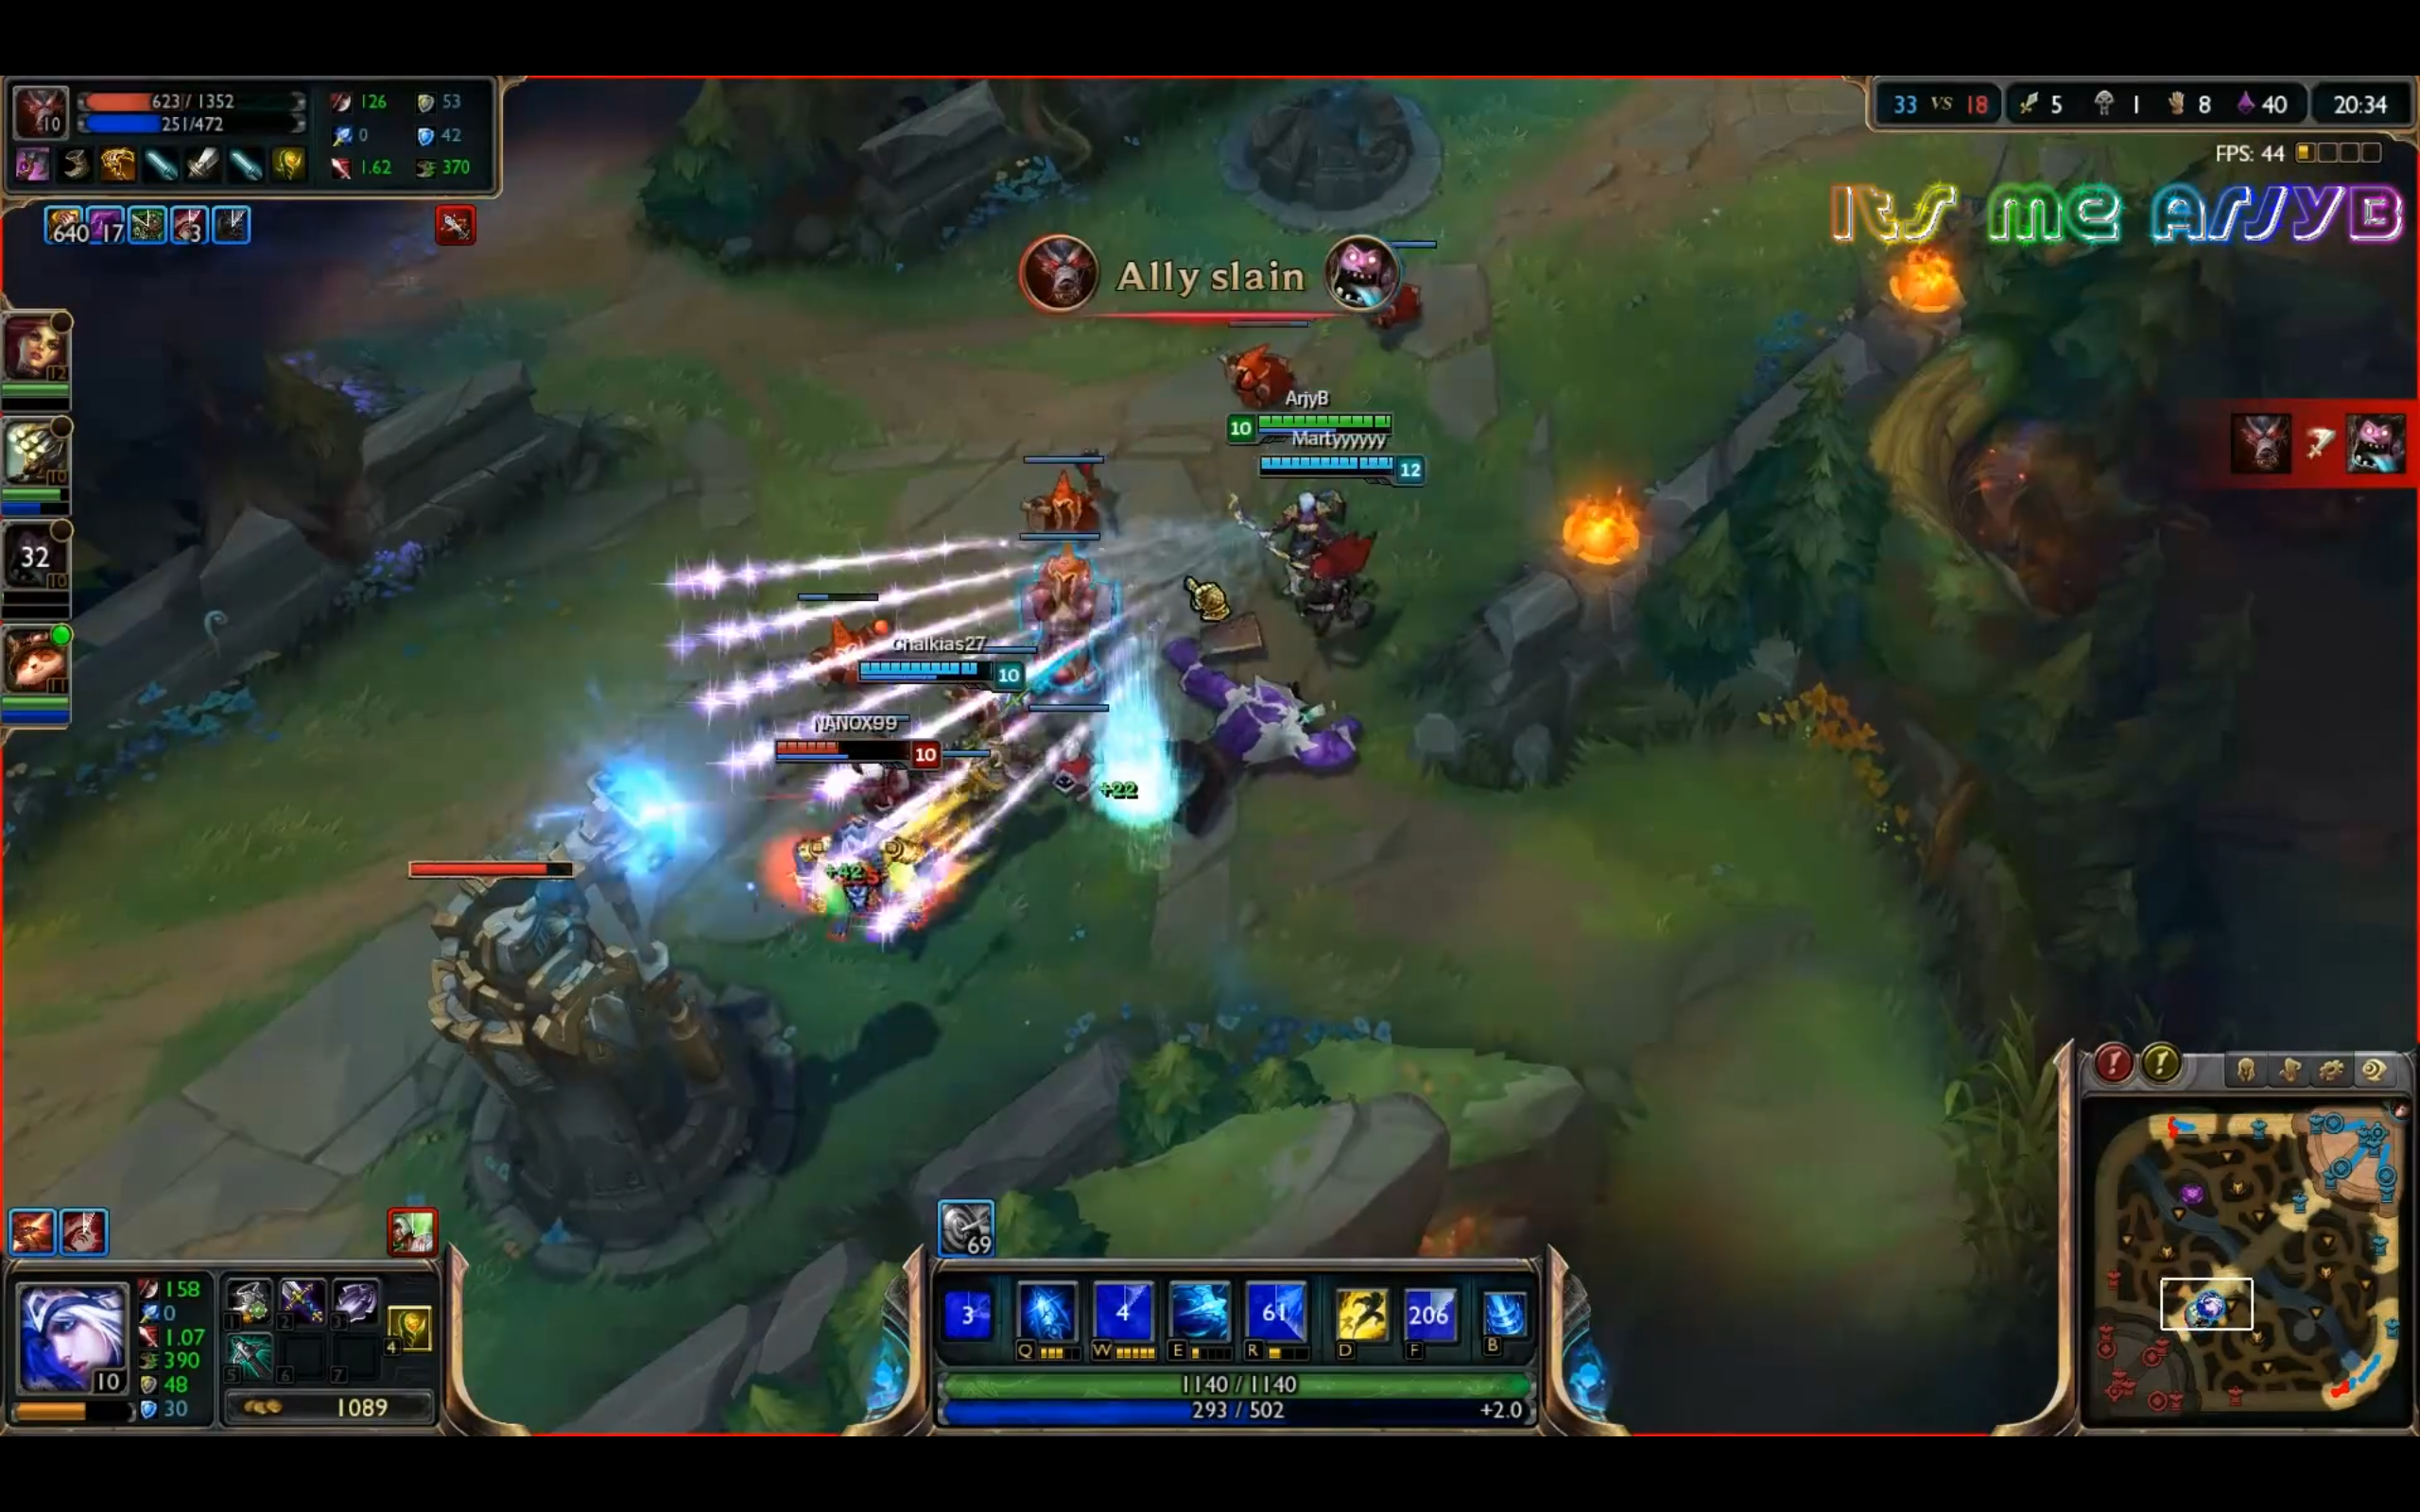
\includegraphics[width=1\textwidth]{img/lolgame.png}
  \caption{Ongoing game: Lower left corner shows the player's chamption equipment and stats. Upper left corner shows a status of friendly champions as well as a summary of a selected champion. Upper right corner shows the current score of the game. The lower right corner shows the map including all structures, friendly units and enemy units in range of friendly units. Lastly in the middle lower screen the champions abilities and health are shown.}\label{fig:lolgame}
\end{figure}

In \Cref{fig:lolgame}, a screenshot of an ongoing game is presented, here the champion \emph{Ashe} uses \emph{Volley} at an enemy player standing near an enemy turret. The description of a subset of Ashe's skills is shown in \Cref{fig:ashe}, including Volley in \Cref{fig:volley}.

\begin{figure}[!htb]
  \centering
  \begin{subfigure}[b]{0.49\textwidth}
    \includegraphics[width=\textwidth]{img/frostshot.png}
    \caption{Example of a passive ability}\label{fig:frostshot}
  \end{subfigure}
  \begin{subfigure}[b]{0.49\textwidth}
    \includegraphics[width=\textwidth]{img/volley.png}
    \caption{Example of an active ability}\label{fig:volley}
  \end{subfigure}
  \begin{subfigure}[b]{0.49\textwidth}
    \includegraphics[width=\textwidth]{img/enchanted.png}
    \caption{Example of an ultimate ability}\label{fig:enchanted}
  \end{subfigure}
  \caption{Subset of Ashe's skillset~\cite{ashe}}\label{fig:ashe}
\end{figure}

The game combines strategy, individual player skill, communication, and team play. With a prize pool exceeding \$2,000,000 in the 2014 LoL World Championships, the game attracts serious and highly skilled players~\cite{lolprize}.


%%% Local Variables:
%%% mode: latex
%%% TeX-master: "../main"
%%% End:
